\documentclass{beamer}

\mode<presentation>
{
	\usetheme{CambridgeUS}
	\setbeamercovered{transparent}
}
\usepackage[spanish]{babel}
\usepackage[latin1]{inputenc}
\usepackage{color}
\usepackage{hyperref}
\usepackage{multicol}
\usepackage{algorithm,algorithmic}

\title[\textbf{ICI 4242 - Aut\'omatas y compiladores}]{\textbf{ICI 4242 - Aut\'omatas y compiladores}}

\subtitle{An\'alisis Sint\'actico}

\author[Rodrigo Olivares]
{
	Rodrigo Olivares \\
	\vspace{0.5mm}
	Mg. en Ingenier\'ia Inform\'atica \\
	\vspace{0.5mm}
	\texttt{\normalsize rodrigo.olivares@uv.cl}
}

\institute[PUCV]

\date{1er Semestre} 

\subject{An\'alisis Sint\'actico}

%\AtBeginSection
%{
%	\begin{frame}<beamer>
%	\frametitle{Contenido}
%	\tableofcontents[currentsection,currentsubsection]
%	\end{frame}
%}
%
%\AtBeginSubsection
%{
%	\begin{frame}<beamer>
%	\frametitle{Contenido}
%	\tableofcontents[currentsection,currentsubsection]
%	\end{frame}
%}
%
%\beamerdefaultoverlayspecification{<+->}

\begin{document}

	\begin{frame}
		\titlepage
	\end{frame}

%	\begin{frame}
%		\frametitle{Contenido}
%		\tableofcontents[pausesections]
%	\end{frame}

	\section{Funciones del analizador sint\'actico}

		%\subsection{Definici\'on}

		\begin{frame}
			\frametitle{Funciones del analizador sint\'actico}
			%\framesubtitle{Definici\'on}

			\begin{block}{Definici\'on}
			    \textbf{Analizador Sint\'actico}: \emph{Corresponde a la segunda fase de un compilador}. En esta fase se construye un \textbf{AST} (\emph{\'arbol de sintaxis abstracta}) para capturar la jerarqu\'ia de la entrada.
			\end{block}
		\end{frame}

		\begin{frame}
			\frametitle{Funciones del analizador sint\'actico}
			%\framesubtitle{Definici\'on}

			\begin{figure}[H]
			    \begin{center}
			        \fbox{\fbox { 
			            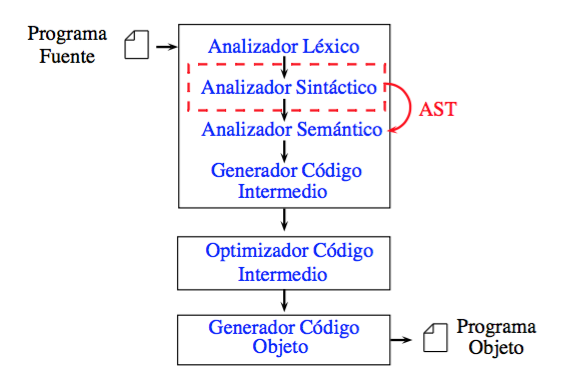
\includegraphics[scale=.45]{images/sin1.png}
			        }}
			    \end{center}
			\end{figure}
		\end{frame}

		\begin{frame}
			\frametitle{Funciones del analizador sint\'actico}

            \begin{block}{}
                \begin{itemize}
                    \item[$\rightarrow$] Construir un \textbf{AST} a partir de los tokens recibidos por el an\'alizador l\'exico.
                \end{itemize}
            \end{block}
			\begin{block}{}
                \begin{itemize}
                    \item[$\rightarrow$] Detecci\'on de \textbf{errores sint\'acticos}.
                \end{itemize}
            \end{block}
            \begin{block}{}
                 \begin{itemize}
                    \item[$\rightarrow$] El analizador sint\'actico tambi\'en se conoce como \textbf{parser}.
                 \end{itemize}
            \end{block}
            \begin{figure}[H]
			    \begin{center}
			        \fbox{\fbox { 
			            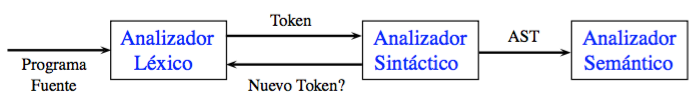
\includegraphics[scale=.45]{images/sin2.png}
			        }}
			    \end{center}
			\end{figure}
		\end{frame}		
		
		\begin{frame}
			\frametitle{Herramientas del analizador sint\'actico}
			%\framesubtitle{Definici\'on}

			\begin{block}{Generadores de analizadores sint\'acticos:}
			 \begin{itemize}
                \item[$\rightarrow$] \textbf{Yacc}
                \item[] (\url{http://dinosaur.compilertools.net/})
                \item[$\rightarrow$] \textbf{Bison}
                \item[] (\url{http://www.gnu.org/software/bison/})
                \item[$\rightarrow$] \textbf{PLY} (Python Lex-Yacc)
                \item[] (\url{http://www.dabeaz.com/ply/})
                \item[$\rightarrow$] \textbf{ANTLR}
                \item[] (\url{http://www.antlr.org/})
                \item[] $\ldots$
			  \end{itemize}
			\end{block}
		\end{frame}

		\begin{frame}
			\frametitle{Implementaci\'on del analizador sint\'actico en ANTLR}
			%\framesubtitle{Definici\'on}

            \begin{block}{}
                \texttt{tokens} \{ \\
			     \hspace{10px} PROGRAM \\
			     \hspace{10px} VAR\_DEC \\
			     \hspace{10px} ASSIGN \\
			     \hspace{10px} $\ldots$ \\
                \} \\
                \vspace{5px}
                \texttt{program} : VAR\_RW! \textbf{var\_dec} BEGIN\_RW! \texttt{body} END\_RW! \\
                \hspace{10px} \{\#\# = \#( \#[PROGRAM, ``PROGRAM''] ,\#\#);\}; \\
                \vspace{5px}
                var\_dec : (type IDENT SEMICOLON!)* \\
                \hspace{10px} \{\#\# = \#( \#[VAR\_DEC, ``VAR\_DEC''] ,\#\#);\}; \\
                \vspace{5px}
                type : NUMERIC\_TYPE $|$ STRING\_TYPE; \\
                \vspace{5px}
                assign : IDENT ASSIG expr SEMICOLON! \\
                \hspace{10px} \{\#\# = \#( \#[ASSIGN, ``ASSIGN"] ,\#\#);\}; \\
			\end{block}
		\end{frame}

		\begin{frame}
			\frametitle{Implementaci\'on del analizador sint\'actico en ANTLR}
			
			\begin{multicols}{2}
			    \begin{table}[H]
			        \begin{center}
			            \begin{tabular}{l}
			                var \\
			                ~~~~ numeric a; \\
			                begin \\
			                ~~~~ a = (a + 1) * b \\
			                end \\
			            \end{tabular}
			        \end{center}
			    \end{table}
			    \begin{figure}[H]
			    \begin{center}
			        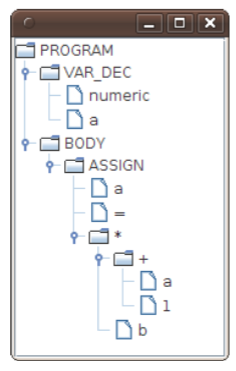
\includegraphics[scale=.55]{images/ast.png}
			    \end{center}
			\end{figure}
			\end{multicols}
	    \end{frame}
	    
	    \begin{frame}
			\frametitle{Implemente el analizador sint\'actico del lenguaje MiLe}

			\begin{block}{Gram\'atica}
                program ::= ``var'' var\_dec ``begin'' body ``end'' \\
                \vspace{5px}
                var\_dec ::= type ident ``;'' \\
                type ::= ``numeric'' $|$ ``string''\\
                \vspace{5px}
                assig ::= ident ``='' exp ``;''\\
                body ::= assig $|$ st $|$ print $|$ read\\
                st ::= for $|$ if\\
            \end{block}
        \end{frame}

	    \begin{frame}
			\frametitle{Implemente el analizador sint\'actico del lenguaje MiLe}

			\begin{block}{Gram\'atica}
                for ::= ``for'' for\_header ``{'' body ``}''\\
                for\_header ::= ``('' assign ``;'' expr ``;'' number ``)''\\
                \vspace{5px}
                if ::= ``if'' ``('' cond ``)'' ``{'' body ``}'' else?\\
                else ::= ``else'' ``{'' body ``}''\\
                \vspace{5px}
                read ::= ``read'' ``('' ident ``)'' ``;''\\
                print ::= ``print'' ``('' string ``,'' ident ``)'' ``;''\\
            \end{block}
        \end{frame}

		\begin{frame}
			\frametitle{Preguntas}

			\hspace{4cm}\huge{Preguntas ?}
		
		\end{frame}
	\end{document}

\usetheme{default}
\usetheme{JuanLesPins}
\usetheme{Goettingen}
\usetheme{Szeged}
\usetheme{Warsaw}

\usecolortheme{crane}

\usefonttheme{serif}
\usefonttheme{structuresmallcapsserif}
 